\begin{figure*}[t]
  \centering
  \begin{subfigure}[b]{\appendixwidth\textwidth}
    \centering
    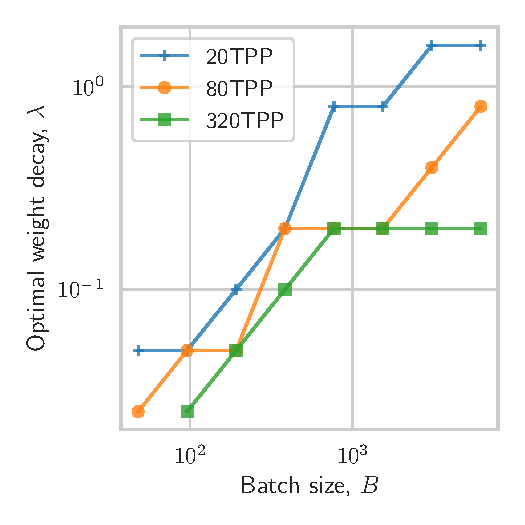
\includegraphics[trim={0.3cm 0.4cm 0.3cm 0.3cm}, clip, width=\linewidth]{pdffigs/batchwise_wds.111M.pdf}
    \caption{111M scale}
    \label{fig:more_wd_scaling_111M}
  \end{subfigure}
  \hfill %
  \begin{subfigure}[b]{\appendixwidth\textwidth}
    \centering
    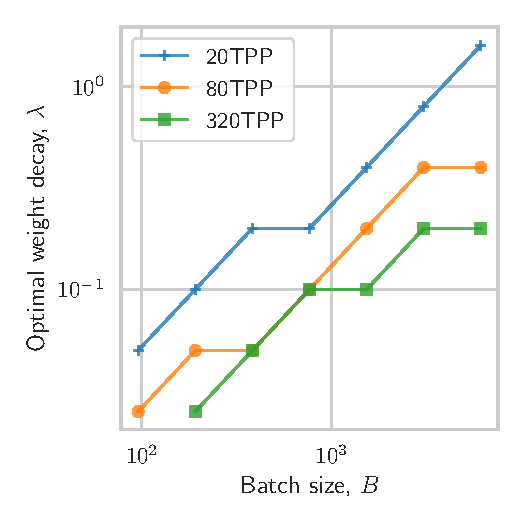
\includegraphics[trim={0.3cm 0.4cm 0.3cm 0.3cm}, clip, width=\linewidth]{pdffigs/batchwise_wds.266M.pdf}
    \caption{266M scale}
    \label{fig:more_wd_scaling_266M}
  \end{subfigure}
  \begin{subfigure}[b]{\appendixwidth\textwidth}
    \centering
    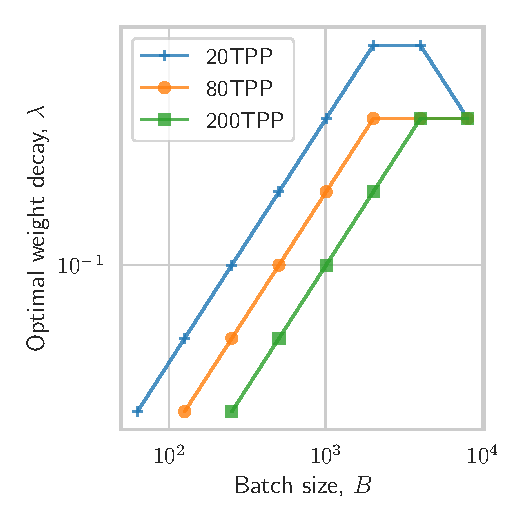
\includegraphics[trim={0.3cm 0.4cm 0.3cm 0.3cm}, clip, width=\linewidth]{pdffigs/batchwise_wds.617M.pdf}
    \caption{610M scale}
    \label{fig:more_wd_scaling_617M}
  \end{subfigure}
  \hfill %
  \begin{subfigure}[b]{\appendixwidth\textwidth}
    \centering
    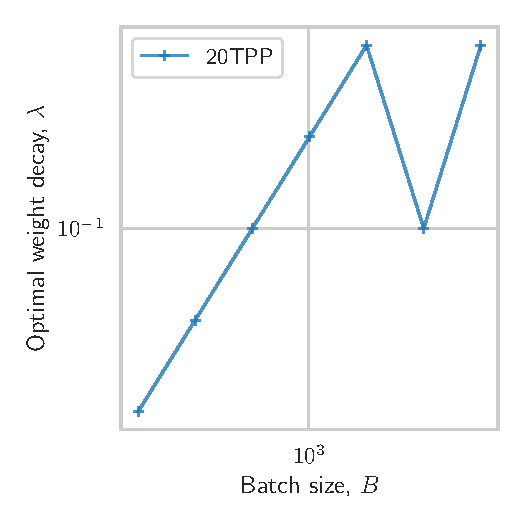
\includegraphics[trim={0.3cm 0.4cm 0.3cm 0.3cm}, clip, width=\linewidth]{pdffigs/batchwise_wds.1.7B.pdf}
    \caption{1.7B scale}
    \label{fig:more_wd_scaling_1_7B}
  \end{subfigure}
  \caption{\textbf{Optimal weight decay scaling with $B$}: The optimal
    weight decay increases linearly over small batch sizes---until
    $B > \cbs$.
    \label{fig:more_wd_scaling}}
\end{figure*}
